
\documentclass[10pt]{article}
\usepackage{amsmath}
\DeclareMathOperator*{\argmin}{arg\,min} % thin space, limits underneath in displays
\DeclareMathOperator*{\argmax}{arg\,max} % thin space, limits underneath in displays
\newtheorem{thm}{Theorem}
\usepackage{amssymb}
\usepackage{amsfonts}
\usepackage{mathrsfs}
\usepackage{bm}
\usepackage{indentfirst}
\setlength{\parindent}{0em}
\usepackage[margin=1in]{geometry}
\usepackage{graphicx}
\usepackage{setspace}
\doublespacing
\usepackage[flushleft]{threeparttable}
\usepackage{booktabs,caption}
\usepackage{float}
\usepackage{graphicx}
\usepackage[sort,comma]{natbib}
\usepackage[hidelinks]{hyperref}

\usepackage{import}
\usepackage{xifthen}
\usepackage{pdfpages}
\usepackage{transparent}

\newcommand{\incfig}[1]{%
\def\svgwidth{\columnwidth}
\import{./figures/}{#1.pdf_tex}
}




\title{IS-LM model}
\author{}
\date{}


\begin{document}
\maketitle



We continue our study of economic fluctuations by looking more closely at aggregate demand. Our goal is to identify the variables that shift the aggregate demand curve, causing fluctuations in national income.

The goal of the model is to show what determines national income for a given price level. There are two ways to interpret this exercise.
\begin{itemize}
\item We can view the IS–LM model as showing what causes income to change in the short run when the price level is fixed because all prices are sticky.
\item Or we can view the model as showing what causes the aggregate demand curve to shift.
\end{itemize}
 


IS stands for “investment” and “saving,” and the IS curve represents what’s going on in the market for goods and services.

LM stands for “liquidity” and “money,” and the LM curve represents what’s happening to the supply and demand for money. 



\section{Building block of IS curve: The Keynesian Cross}
Keynes believed that the problem during recessions and depressions is inadequate spending. The Keynesian cross models this insight.

Identify two concepts:
\begin{itemize}
\item Actual expenditure is the amount households, firms, and the government spend on goods and services. (This is the actual production from firms)
\item Planned expenditure is the amount households, firms, and the government would like to spend on goods and services. (This is the actual sales of, actual demand for,  goods and services.)
\end{itemize}


Therefore, 
\begin{itemize}
\item if actual expenditure $ > $ planned expenditure, firms produce too much, inventory
		is higher. Firms choose to produce less in the next period.
\item if actual expenditure $ < $ planned expenditure, firms produce too less. Consumers
		are eating inventories. Firms choose to produce more in the next period.
\end{itemize}


\subsection{Model set up}
\begin{itemize}
\item The economy is closed, no NX. 
		\begin{equation*}
		PE = C + PI + G
		\end{equation*}

\item Consumption:
		\begin{equation*}
		C = C(Y - T) = A + MPC  \times (Y - T), \text{ MPC: marginal propensity to consume }
		\end{equation*}

\item PI and G are constant:
		\begin{equation*}
		PI =  \overline{PI}, \quad G =  \overline{G}
		\end{equation*}


\item Therefore, 
		\begin{equation*}
		PE = A + MPC  \times (Y - T) +  \overline{PI} +  \overline{G}
		\end{equation*}
\end{itemize}




\subsection{Equilibrium}
In equilibrium, actual expenditure = planned expenditure, i.e., $ Y = PE $

\begin{figure}[H]
\center{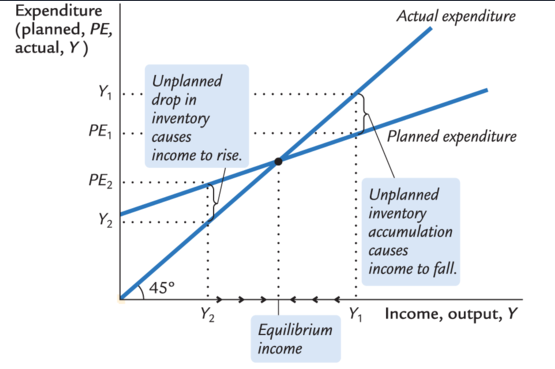
\includegraphics[scale =.5 ]  {figures/equilibrium_keynesian_cross.png}}
\end{figure}



\begin{itemize}
\item When $ Y_1 > PE $, production $ > $  sales, inventory $ \uparrow $, 
		unplanned investment $ \uparrow $, firms produce less in the next period.
\item When $ Y_1 < PE $, production $ < $  sales, inventory $ \downarrow $, 
		unplanned investment $ \downarrow $, firms produce more in the next period.
\end{itemize}



\subsection{Fiscal policy and spending multiplier}
\begin{equation*}
		Y = A + MPC  \times (Y - T) +  \overline{PI} +  \overline{G}  
\end{equation*}
\begin{itemize}
\item A rise in G will first increase Y on the left side.
\item The rise of Y on the left side increases consumption, since C is determined by
		$ (Y - T) $.
\item The rise in C will again foster the growth of Y.
\item Hence, in Keynesian cross, a increase in G leads to a rise of Y that is greater
		than the change in G, i.e., $ \Delta Y > \Delta G $.
\end{itemize}


\subsubsection{Spending multiplier}
\begin{align*}
		Y &= A + MPC  \times (Y - T) +  \overline{PI} +  \overline{G}  \\
		Y &= A + MPC  \times Y  - MPC  \times  T +  \overline{PI} +  \overline{G}  \\
		Y  -  MPC  \times Y &=  \overline{G}  - MPC  \times T + Z, \quad Z = A +  \overline{PI}\\
		(1 - MPC)Y &=  \overline{G} - MPC  \times T + Z\\
		Y&= \frac{1}{1 - MPC}   \times \overline{G} - \frac{MPC}{1 - MPC} \times T + 
		\frac{1}{1 - MPC} \times  Z
\end{align*}
Spending multiplier:
\begin{equation*}
\frac{dY}{dG} = \frac{1}{1 - MPC}
\end{equation*}


\subsubsection{Tax multiplier}
Tax multiplier
\begin{equation*}
\frac{dY}{dT} = -\frac{MPC}{1 - MPC}
\end{equation*}




Effect of change in government spending is greater than change in tax rate, since
the absolute value of spending multiplier is greater than the abs of tax multiplier.

According to an analysis by Obama administration economists, the government-purchases multiplier is 1.57, whereas the tax multiplier is only 0.99.





\section{The goods market and the IS curve}
The Keynesian cross is useful because it shows how the spending plans of households, firms, and the government determine the economy’s income. {\textbf {Yet it makes the simplifying assumption that planned investment I is fixed.}}


In fact, the interest rate and investment are negatively related. Therefore, we write
the planned investment as
\begin{equation*}
I = I(r)
\end{equation*}


{\textbf {Derive the IS curve from graph.}}

\begin{figure}[H]
\center{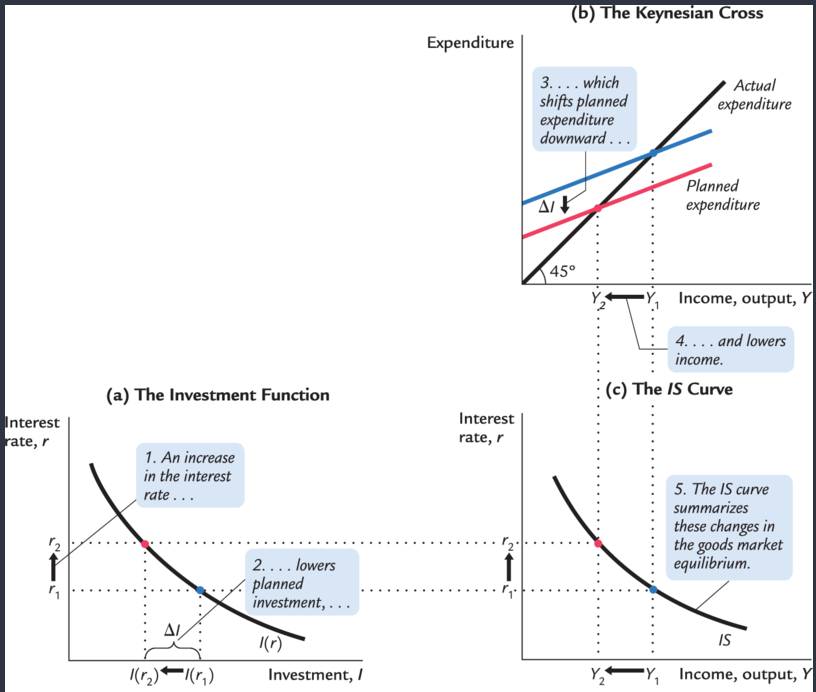
\includegraphics[scale =.5 ]  {figures/derive_IS.png}}
\end{figure}

A rise in interest rate leads to a fall in investment. Planned expenditure falls.
Then, national income falls.

{\textbf {The IS curve summarizes the relationship between the interest rate and 
national income.}}
Each point on the IS curve represents equilibrium in the {\textbf {goods market}}.


\subsection{Fiscal policy and shifts in the IS}


\begin{figure}[H]
\center{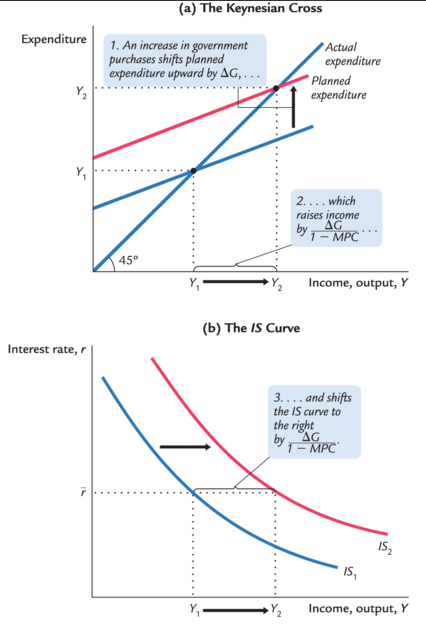
\includegraphics[scale =.6 ]  {figures/fp_and_IS.png}}
\end{figure}




\section{Building block of the LM curve: The Theory of Liquidity Preference}
Define:
\begin{itemize}
\item M, money supply, an exogenous variable, since it is controlled by the central bank.
\item P, price level, an exogenous variable, since we assume {\textbf {P is fixed in the short run}}.
\item $ \frac{M}{P} $, real money balances
\end{itemize}


These imply that the supply of real money balances is fixed and does not depend on
interest rate!

\begin{figure}[H]
\center{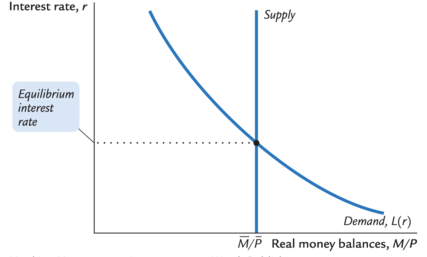
\includegraphics[scale =.6 ]  {figures/money_s_and_d.png}}
\end{figure}




\subsection{Demand for real money balances}
The theory of liquidity preference posits that the interest rate is one determinant of
how much money people choose to hold (demand for money).
Income is {\textbf {another}} determinant of the demand for money.
When income is high, expenditure is high, and people engage in more transactions that
require the use of money.

\begin{equation*}
\left( \frac{M}{P} \right) ^{d} = L(r, Y)
\end{equation*}


\begin{itemize}
\item Interest rate is the opportunity cost of holding money. People earn nothing from
		holding money except for the services provided by money (you can purchase goods using
		money).
\item If $ r $ rises, people hold less money, since they choose to buy more interest-
		bearing assets using their money.
\item If $ r $ falls, people hold more money, since they  interest-bearing assets are
		less attractive.
\end{itemize}



Money demand shifters
\begin{itemize}
\item Income: $ Y \uparrow  \Longrightarrow$ demand for money shift up
\item Restriction on credit card $ \Longrightarrow $ demand for money shift up
\end{itemize}



\subsection{Supply for real money balances}
The supply of real money balances is controlled by the CB.

The supply and demand for real money balances determine what interest rate prevails
in the economy.


\begin{figure}[H]
\center{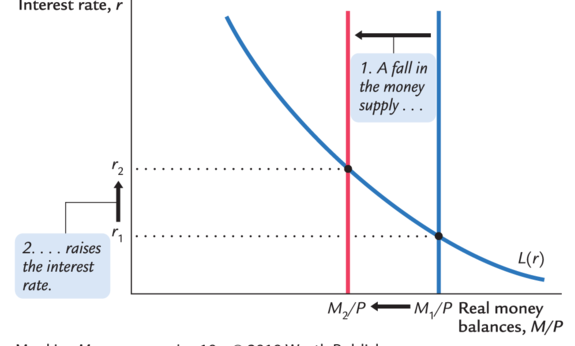
\includegraphics[scale =.6 ]  {figures/money_supply_shift_left.png}}
\end{figure}

Since P is fixed in the short run, when the Fed reduces the money supply M, the supply
of real money balances falls, supply shifts to the left. 
\begin{itemize}
\item It leads to a rise in the equilibrium interest rate.
\item People hold less money and purchase more interest-bearing assets because of the
		higher interest rate.
\end{itemize}



\section{Money market and the LM curve}
The money demand
\begin{equation*}
\left( \frac{M}{P} \right) ^{d} = L(r, Y)
\end{equation*}

is {\textbf {negatively related to the interest rate}} and positively related to income.




\begin{figure}[H]
\center{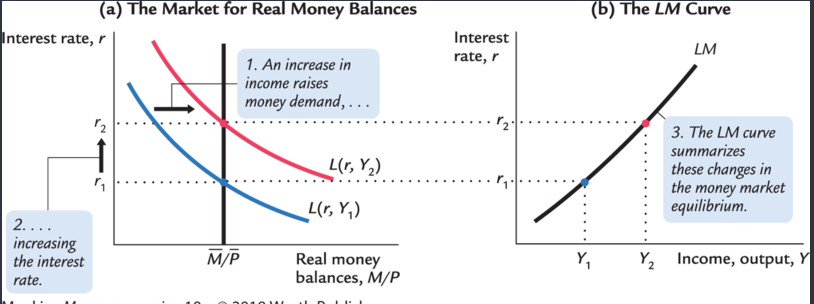
\includegraphics[scale =.6 ]  {figures/money_demand_shifts_right.png}}
\end{figure}



\subsection{Monetary policy and the shift of LM}
Change in income causes a movement along the LM curve.

However, the change in money supply will {\textbf {shift the LM curve}}.

\begin{figure}[H]
\center{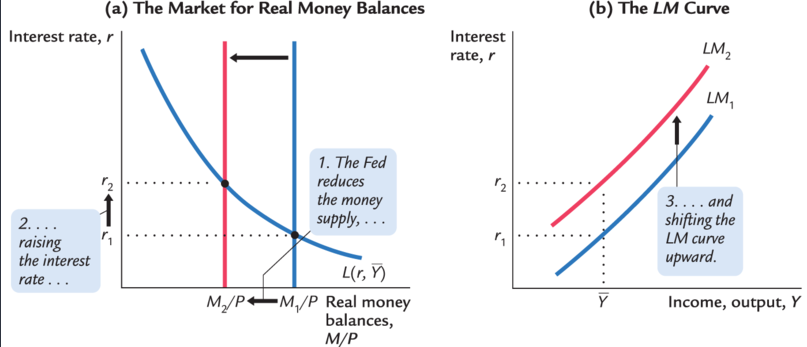
\includegraphics[scale =.6 ]  {figures/money_supply_shift_left_LM.png}}
\end{figure}


\begin{itemize}
\item Decreases in the supply of real money balances shift the LM curve upward.
\item Increases in the supply of real money balances shift the LM curve downward.
\end{itemize}





\section{Equilibrium of IS and LM}
We have the IS curve,
\begin{equation*}
Y = C(Y - T) + I(r) + G,
\end{equation*}
and the LM curve
\begin{equation*}
\frac{M}{P} = L(r, Y)
\end{equation*}

They all posit the relationship between interest rate and national income. The 
intersection of IS and LM determines the equilibrium interest rate and national income. 

In another word, the intersection of IS and LM satisfy conditions for equilibrium in
both goods market and money market.

\begin{figure}[H]
\center{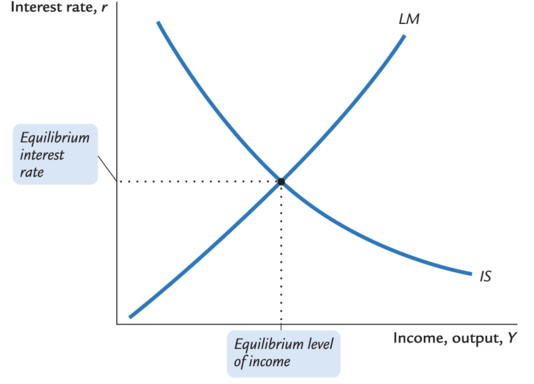
\includegraphics[scale =.6 ]  {figures/IS-LM_equilibrium.png}}
\end{figure}



In summary,

\begin{figure}[H]
\center{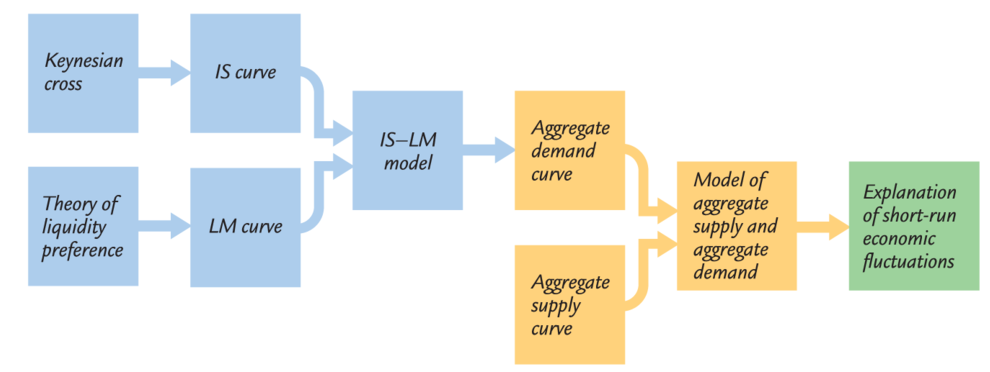
\includegraphics[scale =.5 ]  {figures/blueprint.png}}
\end{figure}





\section{Applying the equilibrium}
Analyze two issues:
\begin{itemize}
\item What are the potential causes of fluctuations in national income Y?
\item How the IS-LM fits into the AD-AS model? (we related the fixed price assumption here)
\end{itemize}


\subsection{Potential causes of fluctuations in national income}

\subsubsection{How fiscal policy affects the short-run equilibrium}
{\textbf {Government purchases:}}

\begin{figure}[H]
\center{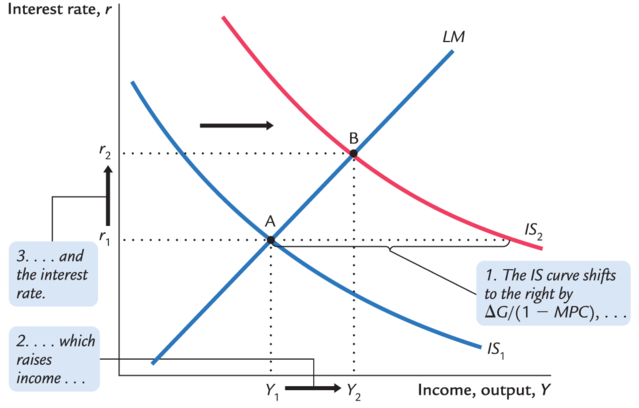
\includegraphics[scale =.6 ]  {figures/fp_equilibrium.png}}
\end{figure}



A rise in G leads to a right shift in the IS curve. In the Keynesian Cross model,
the change in national income Y is {\textbf {greater}} than the change in G because of 
the spending multiplier.


However, in the IS-LM model, the change national income is less than the change in G.

A rise in G leads to an increase in Y. In the money mkt, the rise in Y pushes up the
demand for real money balances while the supply is constant. It causes a rise in the
interest rate.

High interest rate reduces quantity demanded for investment from private sector (the Crowding out effect).


{\textbf {This fall in investment partially offsets the expansion of Y caused by the
rise in G.}}



{\textbf {Tax rate:}}
Same.


\subsubsection{How monetary policy affects the short-run equilibrium}

An increase in M leads to a rise in real money balances, since price is fixed in the 
short run.
\begin{itemize}
\item Rise in real money balances shifts the LM curve to the right.
		\begin{itemize}
		\item interest rate falls, Y rises.
		\end{itemize}
\end{itemize}





\subsubsection{Interaction between monetary and fiscal policy}

A change in one policy may influence the other. For example, suppose Congress raises
taxes.
\begin{itemize}
\item IS shifts to the left $ \Longrightarrow $ interest rate falls, income falls.
\end{itemize}


If the Fed would like to hold the interest rate constant, it needs to reduce the  money
supply causing a left shift in the LM curve (panel b). 
The Fed can hold the interest rate at its previous level. However, the income drops 
further to the left!



If the Fed would like to hold the income constant, it needs to increase the money supply
which causes a righ shift in the LM curve (panel c).
The Fed hold the Y constant while the interest rate drops further.



\begin{figure}[H]
\center{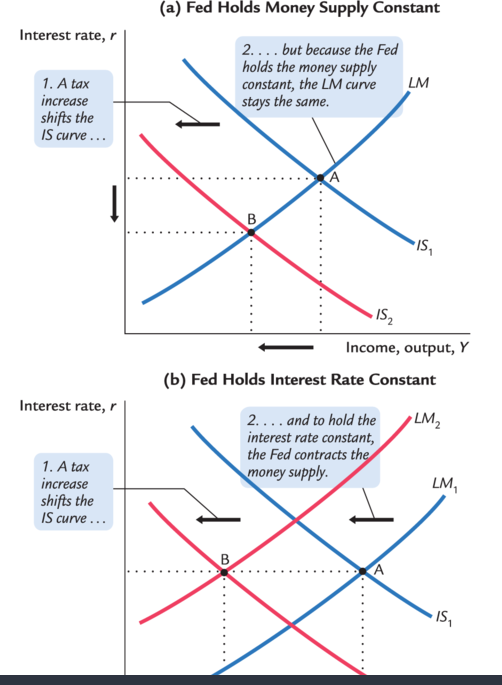
\includegraphics[scale =.6 ]  {figures/fp_mp_together_1.png}}
\end{figure}

\begin{figure}[H]
\center{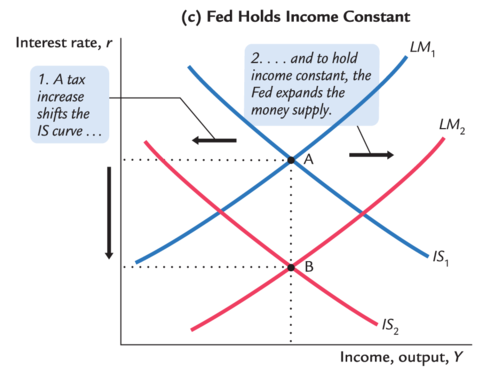
\includegraphics[scale =.6 ]  {figures/fp_mp_together_2.png}}
\end{figure}




\subsubsection{Shocks in the IS-LM model}

{\textbf {Shocks in the IS curve:}}
\begin{itemize}
\item Firms become pessimistic (IS shifts to the left). Income and employment fall.
\item Election of a popular president increases consumer confidence in the economy
		(IS shifts to the right, since consumer spend more.). Income and employment rise.
\item In the recession of 2001, when the optimism on new information technology faded,
		stock prices fall. It {\textbf {reduced}} HHs wealth and thus consumption. (IS
		shifts to the left.)
\item In 2001, the 911 attacks increased uncertainty about what the future world would
		hold. {\textbf {Uncertainty can reduce spending on consumption and investment}} for
		HHs and firms.
\item Accounting scandals at some of the nation's most prominent corporations, e.g.,
		Enron and WorldCom. It discouraged business investment, IS shifts to the left.
\end{itemize}


{\textbf {Shocks in the LM curve (usually arises from exogenous changes in the demand
for money)}}
\begin{itemize}
\item Restriction on credit card(demand for money $ \uparrow $), LM shift to the left.
		\begin{itemize}
		\item In the money market, demand shifts up while supply is constant.
		\item Interest rate is rises.
		\end{itemize}
\end{itemize}




Note, such fluctuations in income are not inevitable. Policymakers can try to use the
tools of monetary and fiscal policy to offset exogenous shocks, if they are sufficiently
quick and skillful. {\textbf {However, they usually not}}!







\subsection{From the IS-LM to the AD}


Before this section, we assume in the SR, price is fixed. 
{\textbf {Now we relax this assumption!}}

For any given money supply $ M $, 
\begin{itemize}
\item a higher price level reduces the supply of real money balances $ \frac{M}{P} $.
		\begin{itemize}
		\item Supply of real money balances shifts to the right $ \Longrightarrow $
				interest rate rises, quantity demanded for investment falls and thus Y.
				({\textbf {interest rate effect}})
		\end{itemize}
\end{itemize}
Hence, the AD curve is downward sloping.

\begin{figure}[H]
\center{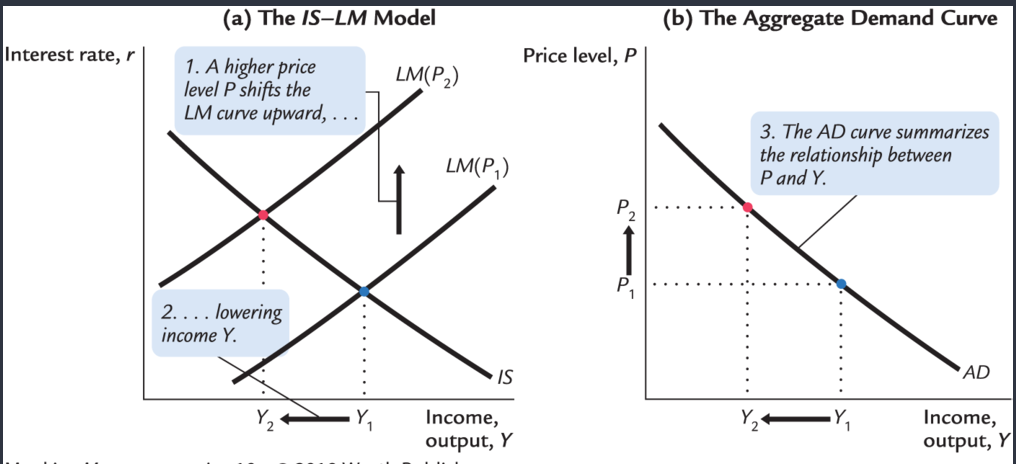
\includegraphics[scale =.5 ]  {figures/LM_to_AD.png}}
\end{figure}






\subsubsection{AD shifters}
Events that shift the IS and LM curve (for a given price level) cause the AD curve to
shift.


Example:
\begin{itemize}
\item Raise in money supply M (expansionary monetary policy)
		\begin{itemize}
		\item LM shift to the right, r falls and Y rises. At any given P, Y rises. 
				It indicates a right shift in the AD curve. (panel a)
		\end{itemize}
\item Increase in G or reduce in T (expansionary fiscal policy)
		\begin{itemize}
		\item Shift the IS to the right and thus AD curve. (panel b)
		\end{itemize}
\end{itemize}



\begin{figure}[H]
\center{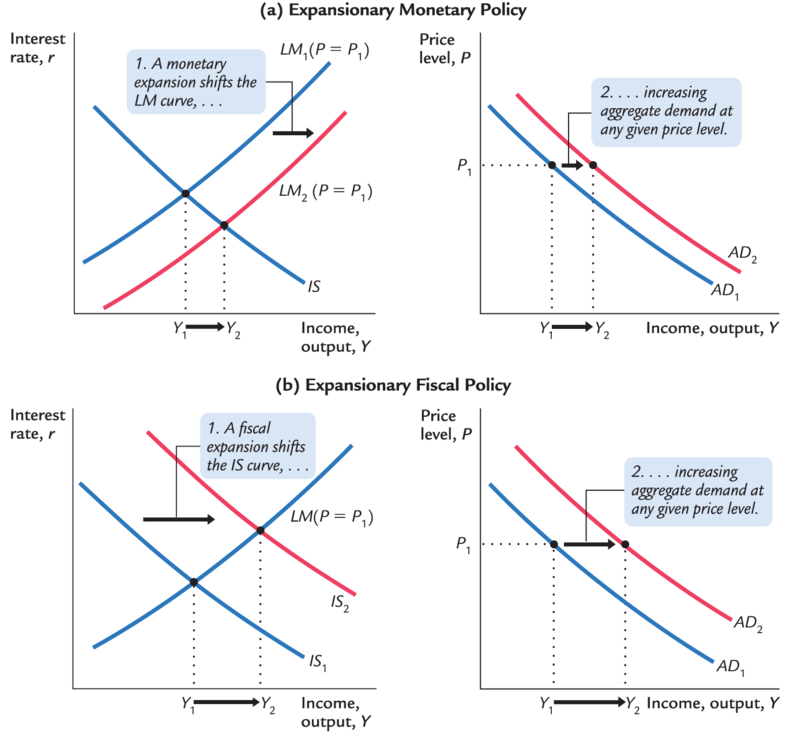
\includegraphics[scale =.6 ]  {figures/AD_shifters.png}}
\end{figure}




\subsection{Keynesian vs. Classical approach}

\begin{figure}[H]
\center{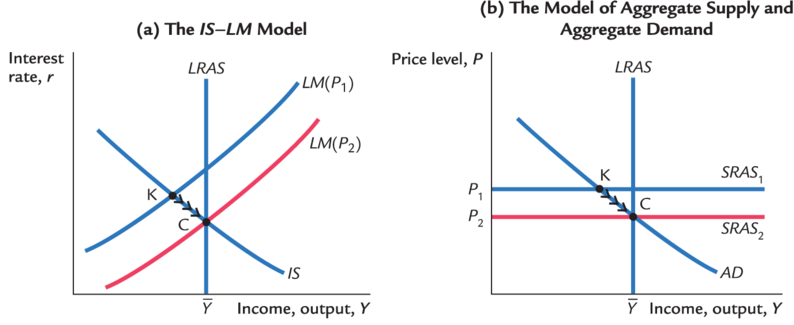
\includegraphics[scale =.6 ]  {figures/keynesian_ISLM_AD.png}}
\end{figure}


Note, according to the Keynesian approach, IS curve is drawn based on fixed price level
while price is allowed to change in LM curve.


Suppose economy starts at SR equilibrium point K. Output is level than the natural
level.
\begin{itemize}
\item In the long run, the low demand for goods and services causes price to fall
		(from $ P_1 $ to $ P_2 $).
\item Then LM shifts to the right, SRAS shifts downward.
\item The economy moves back toward its natural rate.
\end{itemize}




The Keynesian approach assumes price is sticky ({\textbf {P is fixed}}).
\begin{itemize}
\item Output may deviate from its natural level depending on monetary and fiscal policy,
		and other demand shifters.
\item By assuming P is fixed , $ r $ and $ Y $ must adjust to satisfy the IS and LM curve.
		\begin{itemize}
		\item $ P =  \overline{P} $
		\end{itemize}
\end{itemize}




The Classical approach assumes price is flexible. It adjusts to ensure that national
income is {\textbf {always}} at its natural level ($ Y^{*} $)
\begin{itemize}
		\item By assuming $ Y $ is constant ($ Y = Y^{*} $ ), $ r $ and $ P $ must adjust
				to satisfy the IS and LM.
\end{itemize}








\subsection{Expected inflation in the IS-LM model}
Inflation redistribute people wealth. A higher inflation hurts the lender,
and helps the borrower.

The real interest rate is the difference between nominal rate and the expected inflation
rate,
\begin{equation*}
r = i - E \pi.
\end{equation*}

Now the IS curve becomes
\begin{equation*}
IS: \quad Y = C(Y - T) + I(i - E \pi) + G,
\end{equation*}
and the LM is 
\begin{equation*}
LM: \quad \frac{M}{P} = L(i, Y)
\end{equation*}




If people expect the price level to fall in the future, 
\begin{itemize}
\item $ E \pi $ falls.
\item $ r $ rises from $ r_1 $ to $ r_2 $.
\item IS shifts downward.
\item The income falls from $ Y_1 $ to $ Y_2 $
\item The nominal interest rate falls from $ i_1 $ to $ i_2 $.
\end{itemize}

The story behind:
\begin{itemize}
\item When firms come to expect deflation, they become reluctant to borrow to buy investment goods because they believe they will have to repay these loans later in more valuable dollars.
\item The fall in investment depresses planned expenditure, which in turn depresses income.
\item The fall in income reduces the demand for money, and this reduces the nominal interest rate that equilibrates the money market.
\item The nominal interest rate falls by less than the expected deflation, so the real interest rate rises.


\end{itemize}














\bibliographystyle{plainnat}
\bibliography{my_bib}

\end{document}

